\section{Design Model}
\label{sec:Design Model}
Zur elaboration der sechs UC \textit{Import Graph}, \textit{Import Algorithm}, \textit{Delete Graph}, \textit{Delete Algorithm}, \textit{Select Graph} und \textit{Select Algorithm} werden diese je mit den folgenden Diagrammen illustriert:
\begin{itemize}
  \item System Sequence Diagram (SSD): zeigt, wie eine Benutzerinteraktion vom System verarbeitet wird.
  \item Sequence Diagram (SD): zeigt, wie Objekte miteinander arbeiten und erl\"autert die Zust\"andigkeiten der Klassen. 
  \item Design Class Diagram (DCD): zeigt die Elemente des Systems unter Ber\"ucksichtigung ihrer Funktionalit\"at.
\end{itemize}
Jeder System-Event wird mit einer einzigen System-Operation eines Controllers assoziiert. Ein Controller implementiert ausschliesslich System-Operationen (und eventuell einige private Methoden). Generell rufen die Klassen dieses Designs keine Methoden eines Controllers auf.

Anschliessend werden die Konzeptklassen \textit{Parameter Controller} und \textit{Traversal Controller} zur Elaboration als State Machine (SM) betrachtet und je mit einem State Diagram illustriert.
% \newpage
% 
\subsection{UC1 Import Graph}
\begin{figure}[H]
    \centering
    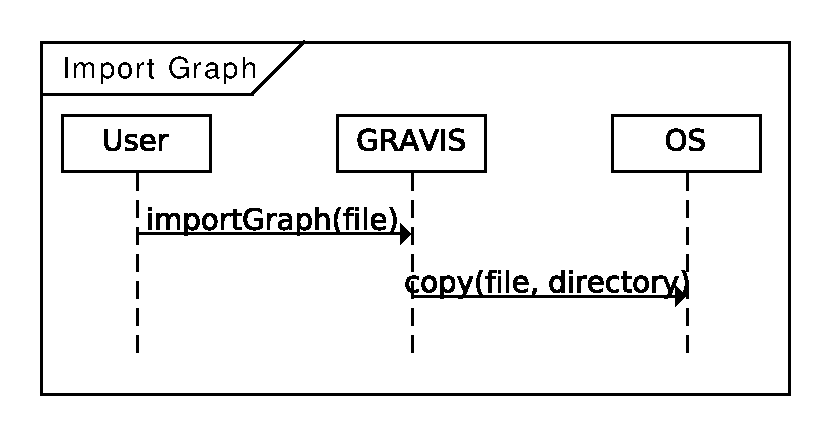
\includegraphics[width=\textwidth]{diagrams/ssd-import-graph.pdf}
    \caption{UC1 Import Graph, System Sequence Diagram}
    \label{fig:import-graph-ssd}
\end{figure}
% \newpage
\begin{figure}
    \centering
    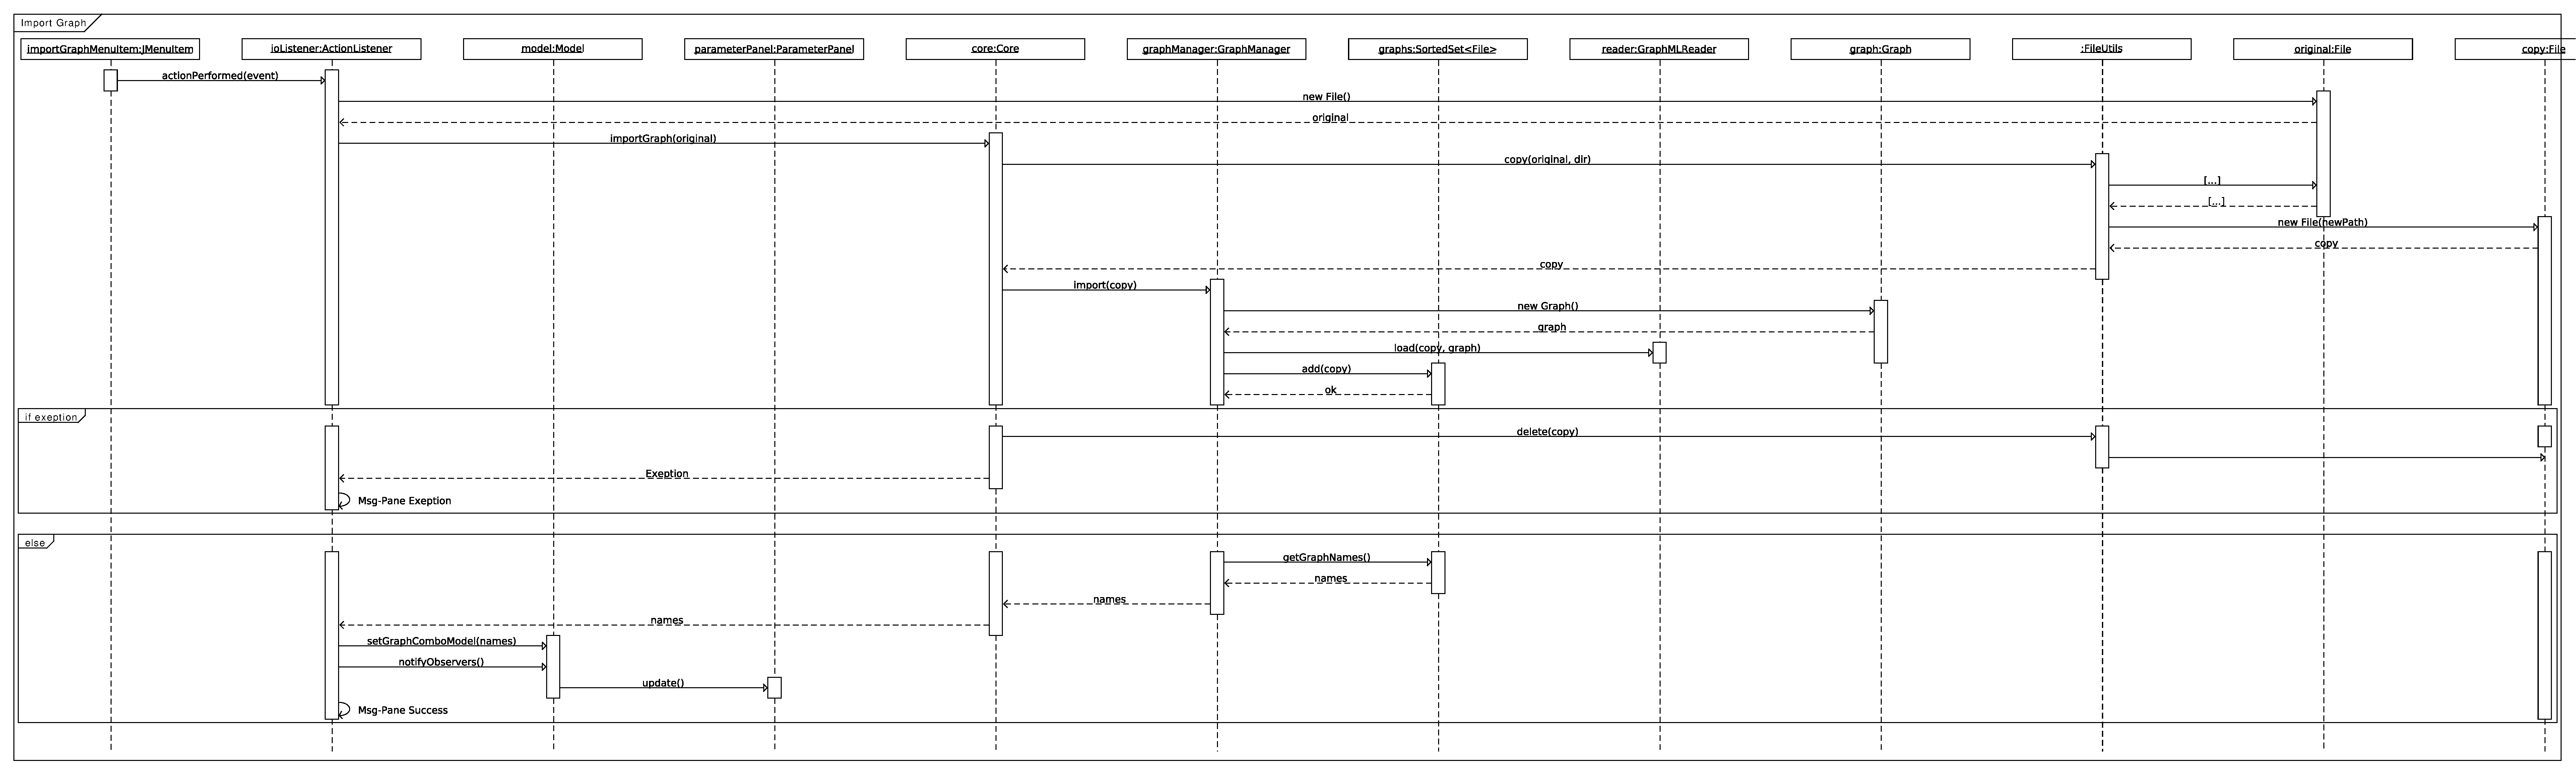
\includegraphics[
% 		    width=\textwidth,
% 		    height=\textheight,
		    angle=90,
		    scale=0.18,
% 		    keepaspectratio=true
	  ]{diagrams/sd-import-graph.pdf}
    \caption{UC1 Import Graph, Sequence Diagram}
    \label{fig:import-graph-sd}
\end{figure}
% \newpage
\begin{figure}[H]
    \centering
    \includegraphics[width=\textwidth]{diagrams/dcd-import-graph.pdf}
    \caption{UC1 Import Graph, Design Class Diagram}
    \label{fig:import-graph-dcd}
\end{figure}
% \newpage
% 
\subsection{UC2 Import Algorithm}
\begin{figure}[H]
    \centering
    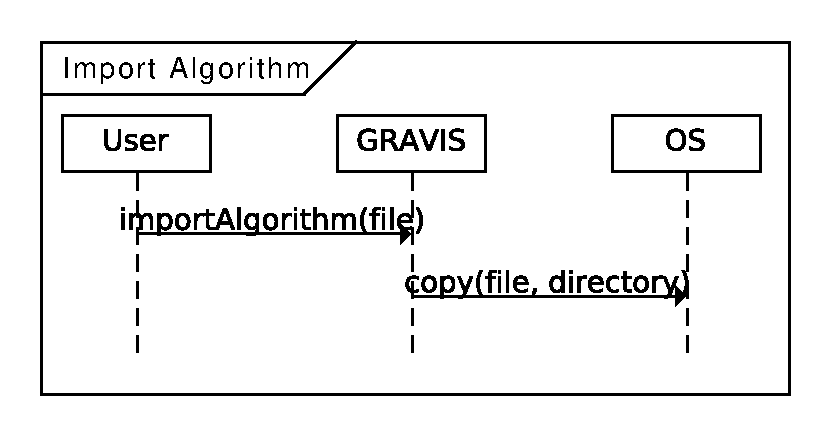
\includegraphics[width=\textwidth]{diagrams/ssd-import-algorithm.pdf}
    \caption{UC2 Import Algorithm, System Sequence Diagram}
    \label{fig:import-algorithm-ssd}
\end{figure}
% \newpage
\begin{figure}[H]
    \centering
    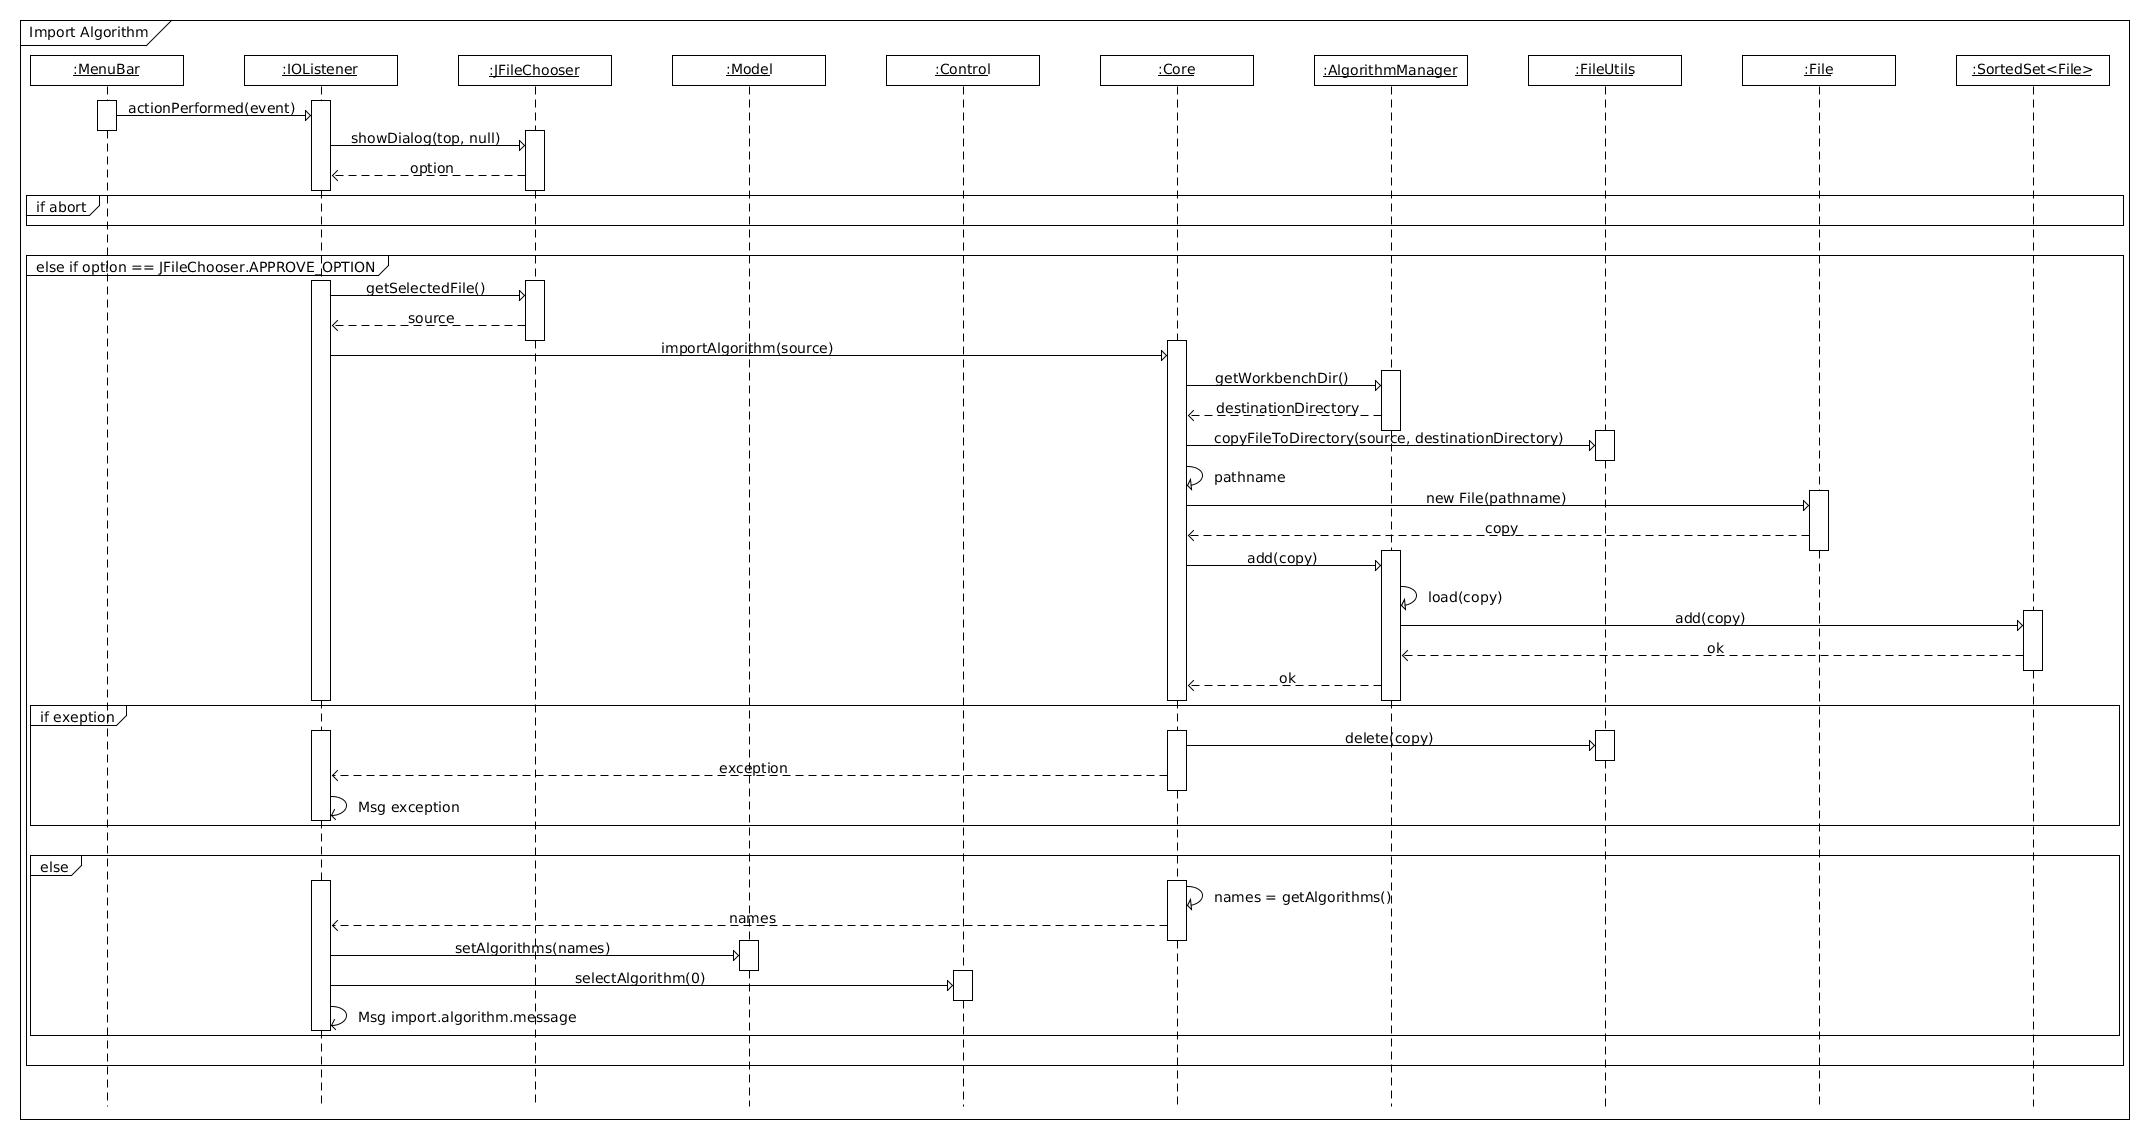
\includegraphics[width=\textwidth]{diagrams/sd-import-algorithm.pdf}
    \caption{UC2 Import Algorithm, Sequence Diagram}
    \label{fig:import-algorithm-sd}
\end{figure}
% \newpage
\begin{figure}[H]
    \centering
    \includegraphics[width=\textwidth]{diagrams/dcd-import-algorithm.pdf}
    \caption{UC2 Import Algorithm, Design Class Diagram}
    \label{fig:import-algorithm-dcd}
\end{figure}
% \newpage
% 
\subsection{UC3 Delete Graph}
\begin{figure}[H]
    \centering
    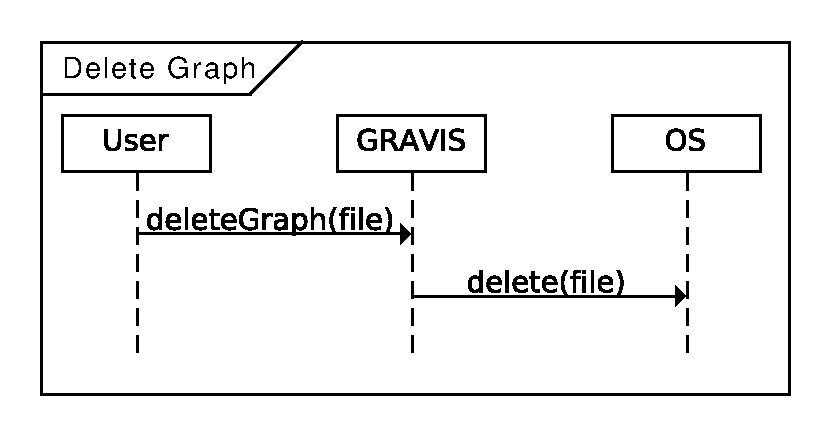
\includegraphics[width=\textwidth]{diagrams/ssd-delete-graph.pdf}
    \caption{UC3 Delete Graph, System Sequence Diagram}
    \label{fig:delete-graph-ssd}
\end{figure}
% \newpage
\begin{figure}[H]
    \centering
    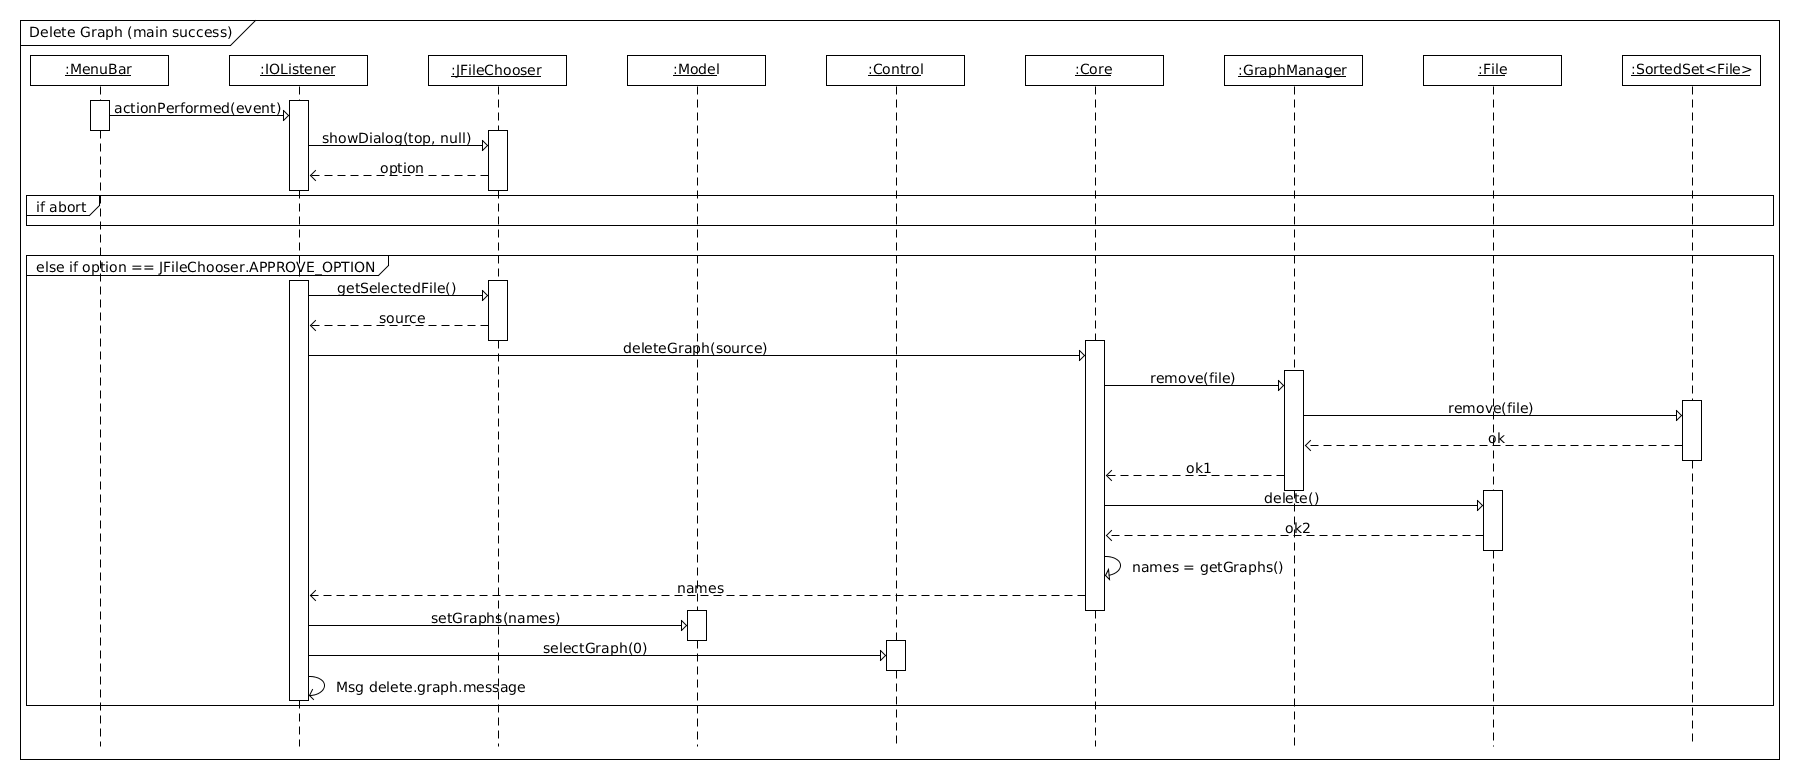
\includegraphics[width=\textwidth]{diagrams/sd-delete-graph.pdf}
    \caption{UC3 Delete Graph, Sequence Diagram}
    \label{fig:delete-graph-sd}
\end{figure}
% \newpage
\begin{figure}[H]
    \centering
    \includegraphics[width=\textwidth]{diagrams/dcd-delete-graph.pdf}
    \caption{UC3 Delete Graph, Design Class Diagram}
    \label{fig:delete-graph-dcd}
\end{figure}
% \newpage
% 
\subsection{UC4 Delete Algorithm}
\begin{figure}[H]
    \centering
    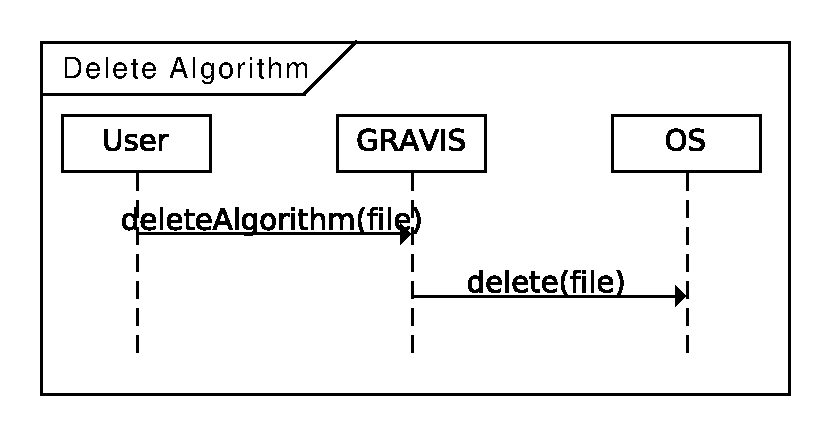
\includegraphics[width=\textwidth]{diagrams/ssd-delete-algorithm.pdf}
    \caption{UC4 Delete Algorithm, System Sequence Diagram}
    \label{fig:delete-algorithm-ssd}
\end{figure}
% \newpage
\begin{figure}[H]
    \centering
    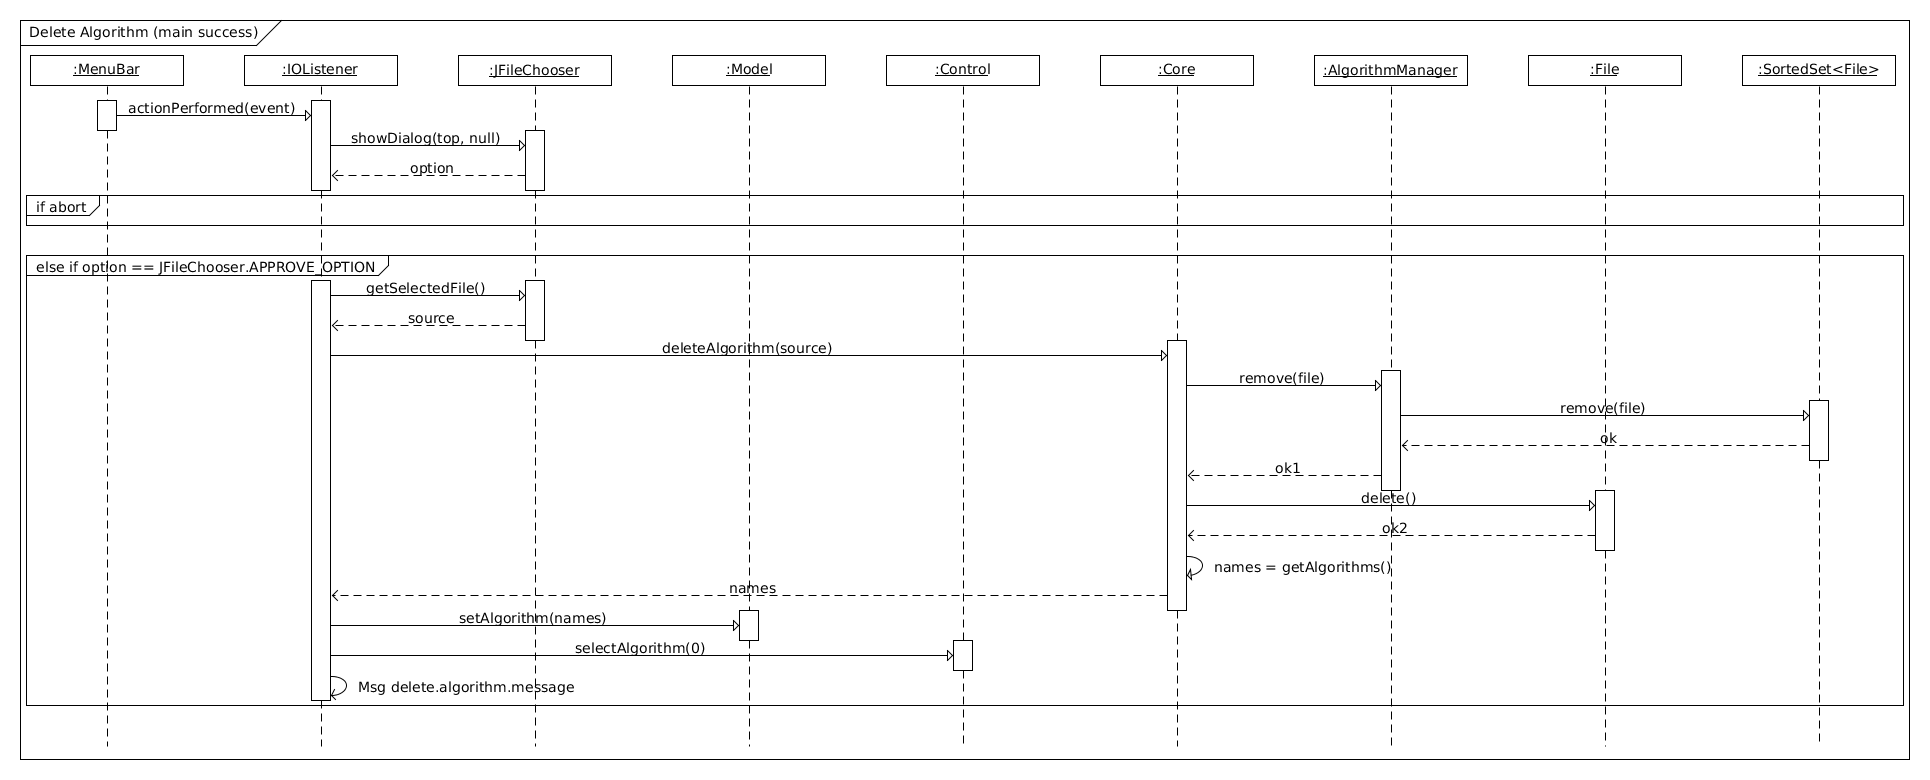
\includegraphics[width=\textwidth]{diagrams/sd-delete-algorithm.pdf}
    \caption{UC4 Delete Algorithm, Sequence Diagram}
    \label{fig:delete-algorithm-sd}
\end{figure}
% \newpage
\begin{figure}[H]
    \centering
    \includegraphics[width=\textwidth]{diagrams/dcd-delete-algorithm.pdf}
    \caption{UC4 Delete Algorithm, Design Class Diagram}
    \label{fig:delete-algorithm-dcd}
\end{figure}
% \newpage
% 
\subsection{UC5 Select Graph}
\begin{figure}[H]
    \centering
    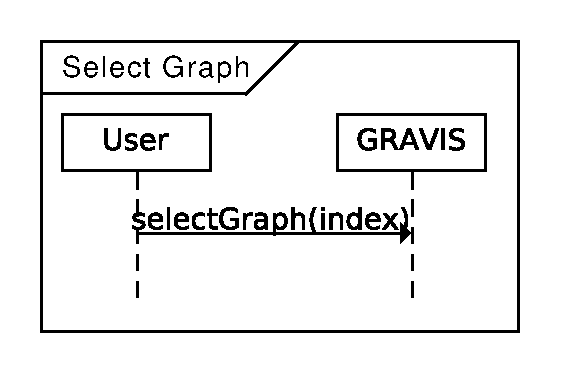
\includegraphics[width=\textwidth]{diagrams/ssd-select-graph.pdf}
    \caption{UC5 Select Graph, System Sequence Diagram}
    \label{fig:select-graph-ssd}
\end{figure}
% \newpage
\begin{figure}[H]
    \centering
    \includegraphics[width=\textwidth]{diagrams/sd-select-graph.pdf}
    \caption{UC5 Select Graph, Sequence Diagram}
    \label{fig:select-graph-sd}
\end{figure}
% \newpage
\begin{figure}[H]
    \centering
    \includegraphics[width=\textwidth]{diagrams/dcd-select-graph.pdf}
    \caption{UC5 Select Graph, Design Class Diagram}
    \label{fig:select-graph-dcd}
\end{figure}
% \newpage
% 
\subsection{UC6 Select Algorithm}
\begin{figure}[H]
    \centering
    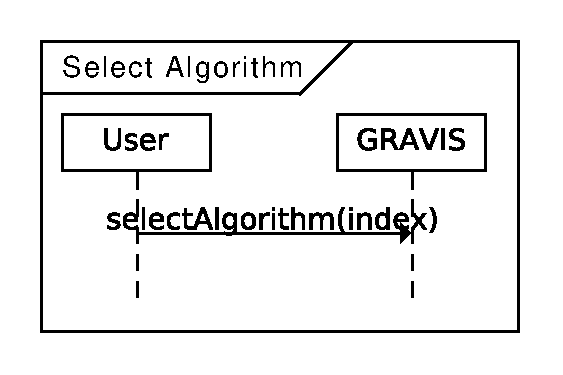
\includegraphics[width=\textwidth]{diagrams/ssd-select-algorithm.pdf}
    \caption{UC6 Select Algorithm, System Sequence Diagram}
    \label{fig:select-algorithm-ssd}
\end{figure}
% \newpage
\begin{figure}[H]
    \centering
    \includegraphics[width=\textwidth]{diagrams/sd-select-algorithm.pdf}
    \caption{UC6 Select Algorithm, Sequence Diagram}
    \label{fig:select-algorithm-sd}
\end{figure}
% \newpage
\begin{figure}[H]
    \centering
    \includegraphics[width=\textwidth]{diagrams/dcd-select-algorithm.pdf}
    \caption{UC6 Select Algorithm, Design Class Diagram}
    \label{fig:select-algorithm-dcd}
\end{figure}
% \newpage
% 
\subsection{Parameter Controller}
\begin{figure}[H]
    \centering
    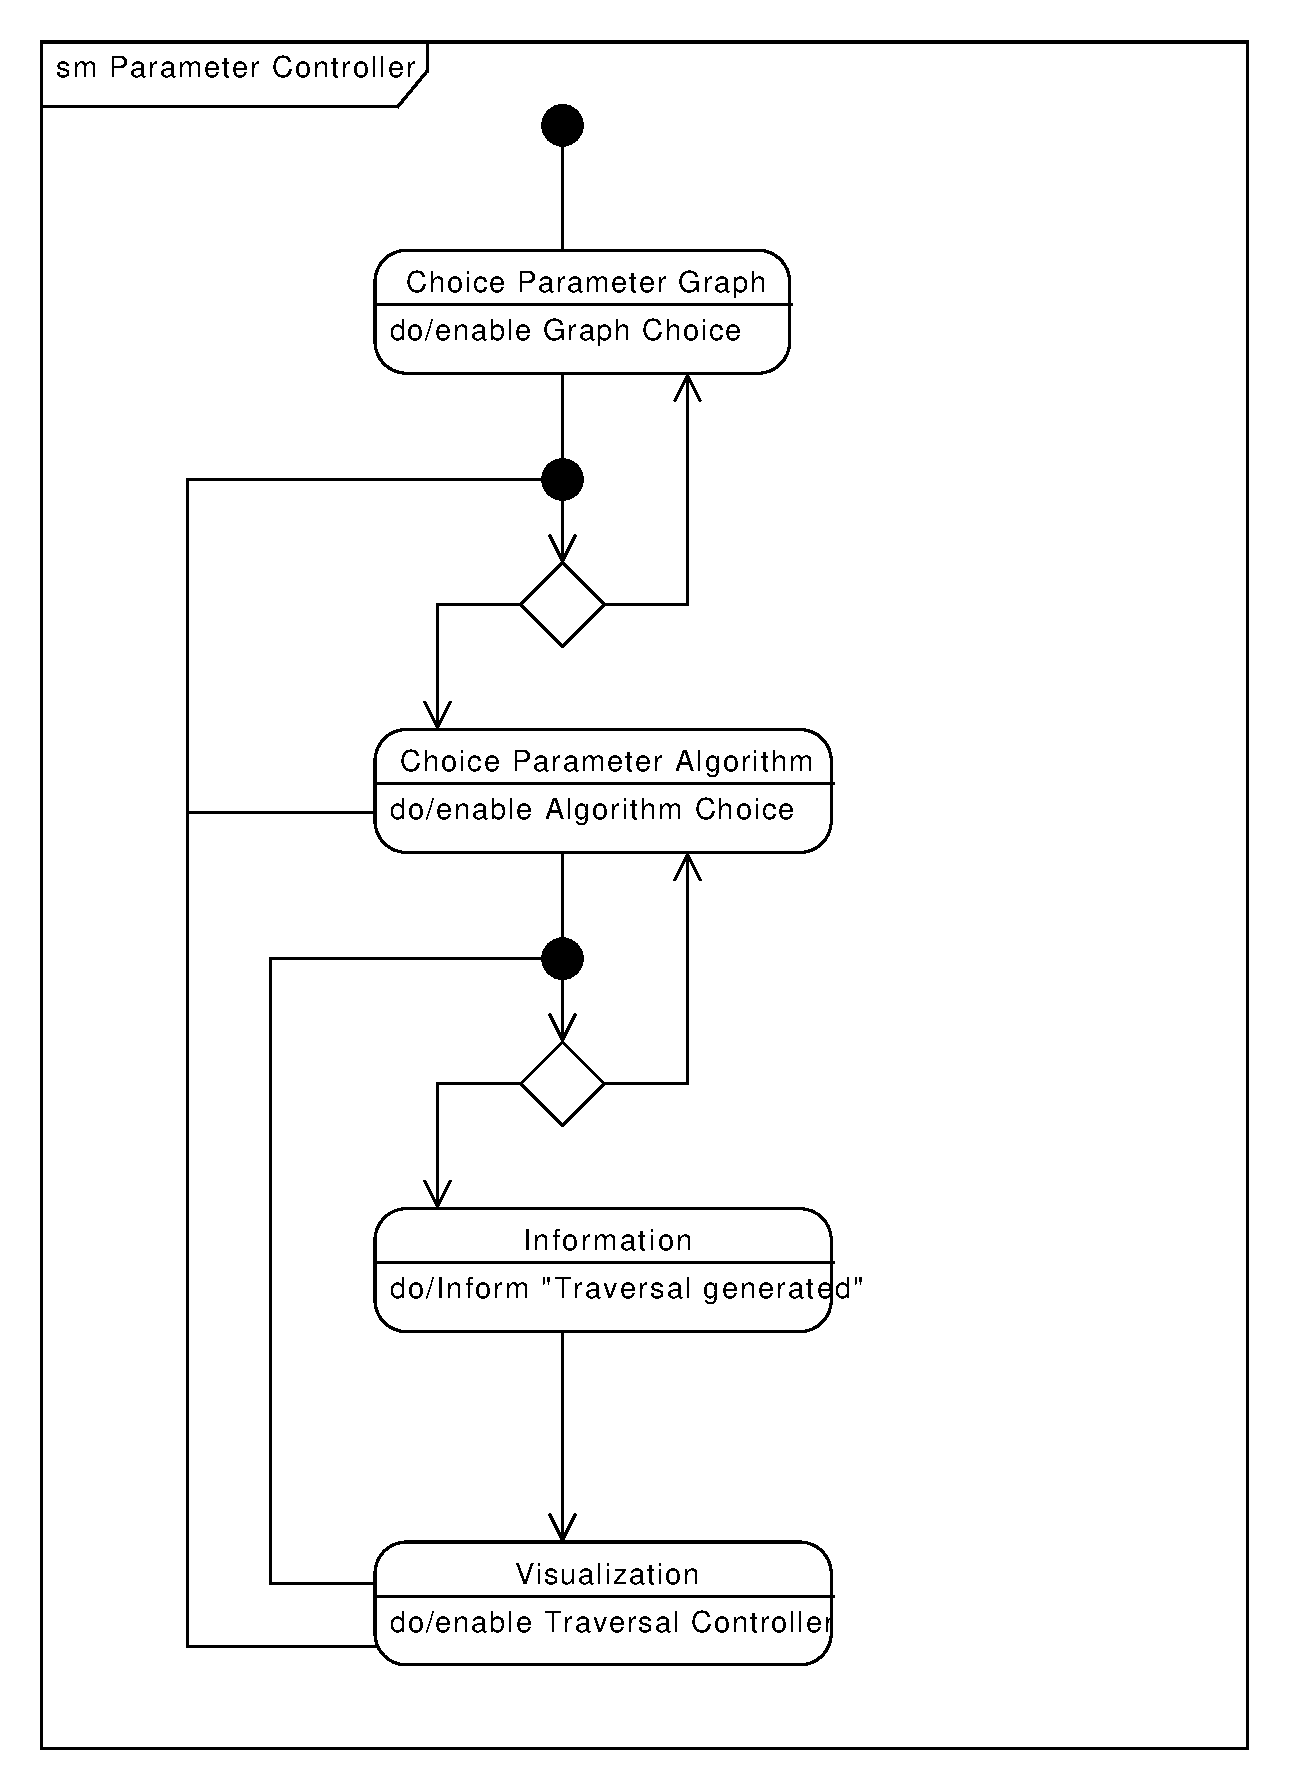
\includegraphics[width=\textwidth]{diagrams/sm-parameter-controller.pdf}
    \caption{Parameter Controller, State Diagram}
    \label{fig:sm-parameter-controller}
\end{figure}
% \newpage
% 
\subsection{Traversal Controller}
\begin{figure}[H]
    \centering
    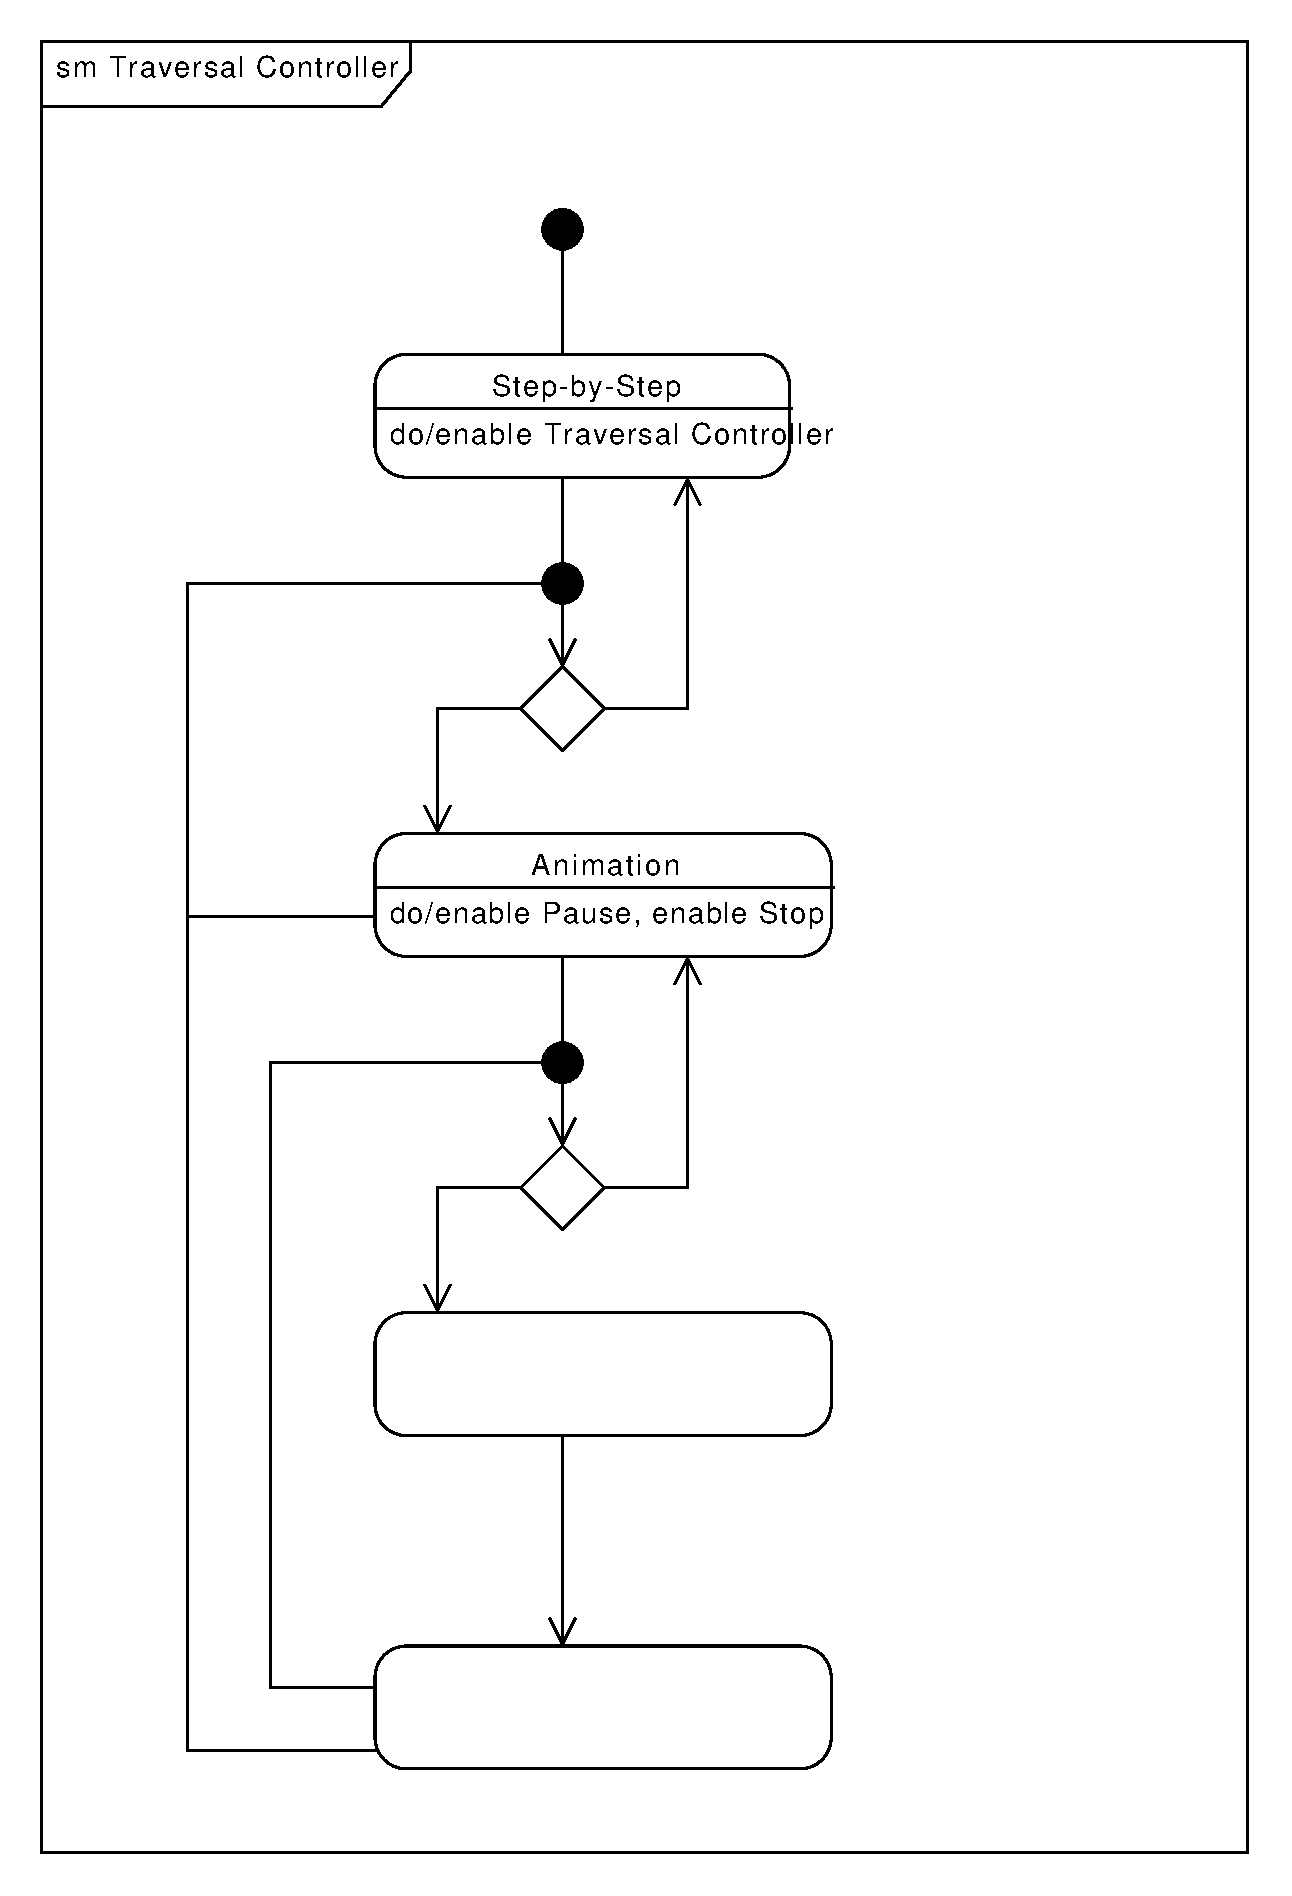
\includegraphics[width=\textwidth]{diagrams/sm-traversal-controller.pdf}
    \caption{Traversal Controller, State Diagram}
    \label{fig:sm-traversal-controller}
\end{figure}